\documentclass[conference]{IEEEtran}
\usepackage[numbers,sort]{natbib}

\ifCLASSINFOpdf
  % \usepackage[pdftex]{graphicx}
  % declare the path(s) where your graphic files are
  % \graphicspath{{../pdf/}{../jpeg/}}
  % and their extensions so you won't have to specify these with
  % every instance of \includegraphics
  % \DeclareGraphicsExtensions{.pdf,.jpeg,.png}
\else
  % or other class option (dvipsone, dvipdf, if not using dvips). graphicx
  % will default to the driver specified in the system graphics.cfg if no
  % driver is specified.
  % \usepackage[dvips]{graphicx}
  % declare the path(s) where your graphic files are
  % \graphicspath{{../eps/}}
  % and their extensions so you won't have to specify these with
  % every instance of \includegraphics
  % \DeclareGraphicsExtensions{.eps}
\fi

% correct bad hyphenation here
\hyphenation{op-tical net-works semi-conduc-tor}

\usepackage{pdfpages}
\usepackage[export]{adjustbox}

\begin{document}
%
% paper title
% can use linebreaks \\ within to get better formatting as desired
% Do not put math or special symbols in the title.
\title{Opportunistic Network Simulation}

% author names and affiliations
% use a multiple column layout for up to three different
% affiliations
\author{
\IEEEauthorblockN{Vojtech Miksu, Nils Gustav Davidsson, Drew Carrington, Jiayu Chen, Anjjan Narayan}
\IEEEauthorblockA{College of Computing\\
Georgia Institute of Technology\\
Atlanta, Georgia 30332\\
Email: \{miksu, gustav, dcarrington3, jychen, anjjan.narayan\}@gatech.edu}
}

% make the title area
\maketitle

% As a general rule, do not put math, special symbols or citations
% in the abstract
\begin{abstract} % Please feel free to edit this
With the increasing use of mobile devices and vehicular networking, ad-hoc networking sees increasingly interesting applications. Since there are often no end-to-end connections at any given time, opportunistic networking is sometimes the best option in rural areas, during disaster relief, in certain military situations and more. We found that it would be valuable to compare prominent opportunistic networks protocols. We have done this using the ONE simulator and a map of the campus of Georgia Institute of Technology, and evaluated the schemes with regard to message delivery probability, energy efficiency, and more.
\end{abstract}

% As a general rule, do not put math, special symbols or citations
% in the abstract
\begin{keywords}
The ONE; opportunistic networks; routing
\end{keywords}

% For peerreview papers, this IEEEtran command inserts a page break and
% creates the second title. It will be ignored for other modes.
\IEEEpeerreviewmaketitle

\section{Introduction}
% no \IEEEPARstart

With the increasing use of mobile devices such as smart phones, tablets and laptop computers that are connected wirelessly to a network, there arises a potential to use ad-hoc networks. Ad-hoc networks are the only option for some applications where various challenges such as intermittent connectivity and variable performance arise. In most cases these networks do not contain a path from source to destination.

Opportunistic network provides the perfect platform to improve the usability and connectivity of mobile devices that are on the go. Our work primarily focuses on opportunistic network protocols. As a part of our work, we compare the different protocols, their parameterization and ultimately come up with our proposal and implementation of enhancement to the protocols. During the study, we use The Opportunistic Networks Environment (The ONE) simulator \cite{keranen-theone} that was created at Helsinki University of Technology.

The ONE is a complex tool that enables a real-time simulation of delay-tolerant networks. It implements various existing protocols and provides an interface to create and test new ones. It is also possible to use different map backgrounds since opportunistic networks are heavily related to a real-world routes. We use a map of Georgia Tech in Atlanta.

% An example of a floating figure using the graphicx package.
% Note that \label must occur AFTER (or within) \caption.
% For figures, \caption should occur after the \includegraphics.
% Note that IEEEtran v1.7 and later has special internal code that
% is designed to preserve the operation of \label within \caption
% even when the captionsoff option is in effect. However, because
% of issues like this, it may be the safest practice to put all your
% \label just after \caption rather than within \caption{}.
%
% Reminder: the "draftcls" or "draftclsnofoot", not "draft", class
% option should be used if it is desired that the figures are to be
% displayed while in draft mode.
%
%\begin{figure}[!t]
%\centering
%\includegraphics[width=2.5in]{myfigure}
% where an .eps filename suffix will be assumed under latex,
% and a .pdf suffix will be assumed for pdflatex; or what has been declared
% via \DeclareGraphicsExtensions.
%\caption{Simulation Results.}
%\label{fig_sim}
%\end{figure}

% Note that IEEE typically puts floats only at the top, even when this
% results in a large percentage of a column being occupied by floats.

% An example of a double column floating figure using two subfigures.
% (The subfig.sty package must be loaded for this to work.)
% The subfigure \label commands are set within each subfloat command,
% and the \label for the overall figure must come after \caption.
% \hfil is used as a separator to get equal spacing.
% Watch out that the combined width of all the subfigures on a
% line do not exceed the text width or a line break will occur.
%
%\begin{figure*}[!t]
%\centering
%\subfloat[Case I]{\includegraphics[width=2.5in]{box}%
%\label{fig_first_case}}
%\hfil
%\subfloat[Case II]{\includegraphics[width=2.5in]{box}%
%\label{fig_second_case}}
%\caption{Simulation results.}
%\label{fig_sim}
%\end{figure*}
%
% Note that often IEEE papers with subfigures do not employ subfigure
% captions (using the optional argument to \subfloat[]), but instead will
% reference/describe all of them (a), (b), etc., within the main caption.

\section{Opportunistic networks}

In order to avoid the costly process of introducing cables into a building, or as a connection between various equipment locations, personal devices, telecommunication networks and business installations are moving to wireless networks. The devices such as smart phones, tablets and laptops are in constant movement from one location to another. There is no solid infrastructure or protocols that can manage this transition of devices from one location to another.

During the last few years, ad hoc networks have been studied extensively and implemented on various application environments. As the application environments of these networks keep increasing, their traditional techniques and approaches need some improvements. One of the recent evolution in ad hoc networks is Mobile ad hoc networks (MANETs). Ad hoc networks also helps mobile nodes to reach infrastructure when some node in the network acts as a gateway. However, if the density of the nodes increases or the connection of a node in the network breaks, traditional network protocols would not be able to provide means for connection establishment and communication.

Wireless network properties such as disconnection of nodes, mobility of users, and link instability cannot be handled in traditional networks. Opportunistic networks are created for mobile devices without relying on pre-existing topology. Opportunistic networks are the evolution of MANETs. In opportunistic networks, mobile nodes can communicate with each other even if a route connecting them does not exist. Opportunistic networks consists of a variety of applications. Some of the applications include opportunistic computing, mobile data offloading, recommender systems etc. Opportunistic networks are created out of mobile devices carried by people, without relying on any existing network topology. In opportunistic network mobility is used as a technique to provide communication between disconnected nodes, rather than a drawback to be solved. Opportunistic networks can be useful for emergency broadcasts, vehicle-to-vehicle communication.



\section{Opportunistic Network Protocols}
Routing protocols in opportunistic networks are based on the ability to transfer data or message from source to destination. Opportunistic networks are characterized based on lack of connectivity between the nodes and lack of direct end-to-end paths. Routing protocols are designed to handle these exceptions. There are various opportunistic network routing protocols. For our experiment, we have used the following protocols.

\subsection{Epidemic Routing}  
Epidemic routing [reference added to ref.bib] is a subclass of flooding. In this protocol nodes replicate the message in a continuous manner and transmit the message to the nodes that are newly discovered. The message is transferred to the newly discovered nodes only if the new node does not already have the message. There are various methods that can be used to limit the number of replications in the network. Epidemic routing provides delivery of the message to random destinations with minimum assumption of the network connectivity. The final delivery of the message depends on the connectivity of the nodes. 

Epidemic routing works on the theory of epidemic algorithms. The host contains two buffers to store the messages that it originated and the messages that it is buffering on behalf of other hosts. There is also a summary vector in each hosts that describes the order of messages in the stored buffer. When two hosts are in contact, they exchange their summary vector to check if the new message already exists. If not, the message is transferred. 

In our implementation of epidemic routing protocol, we have used drop-oldest buffer technique. When the buffer is full, the oldest message is dropped to accommodate the new message. Also, the protocol uses single transferring connection at a time. 

\subsection{PRoPHET Routing}
Probabilistic Routing Protocol using History of Encounters and Transitivity (PRoPHET) [ reference in ref.bib third item]makes use of an assumption that If a user has visited a location several times before, there is more probability to visit that location again. Unlike epidemic routing, PRoPHET assumes that nodes move in a periodic fashion. PRoPHET uses an algorithm to exploit this periodic movement of nodes by assigning a set of probabilities for successful delivery to a known destination. It also replicates the message during opportunistic encounter only if the node that doesn't have the message has a better chance of delivering it.     

\subsection{Spray and Wait Protocol}
The main idea behind spray and wait protocol [ reference in ref.bib fourth item] is that it achieves resource efficiency by setting a threshold value on the number of copies of a message allowed in a network.
As the name suggests, spray and wait contains two phases, the spray phase and the wait phase. Everytime a new message is created in the system, a number X is attached to the message. X indicates the maximum number of copies of the message that is allowed in the network. In the spray phase, the host node sprays one copy of the message to X nodes in the network. When a node receives the message, it enters the wait phase. In the wait phase the node waits until it achieves direct communication with the destination. Once it does, it sends the copy of the message to the destination node.   

\subsection{Direct Routing Protocol}
Direct routing protocol is a simple protocol that is based on direct contact between the source and the destination node. The source node which generates the message will transmit the message to the destination node only if there is a direct connection between source and destination. The message will not pass through intermediate nodes. 

\subsection{First Contact Protocol}
First contact protocol is another simple protocol which is based on nodes that are first contact to the host node. The host node generates a single copy of the message. This single copy is sent across all the nodes and no other copies are made. A source node will send the copy of the message to the nodes that is a first available contact to the host node. Similar pattern is followed by other nodes until the message reaches the destination node. 



\section{The one simulator}

For the project, we are mainly working with the Opportunistic Network Simulator (ONE). ONE is an event simulation engine which is used to model node movement, inter-node connections using various interfaces, routing, message handling and application interactions. The simulator also provides tools for visualization, reports and post-processing tools.

Node movement is implemented using movement models which are either synthetic or movement traces. Nodes are connected based on their location, communication-range or bit-rate. The routing models decide which messages to forward over the existing connections. The messages are generated either through event generators (to generate random traffic between nodes) or through applications that generate traffic based on application interactions.

\section{Background map}

The ONE simulator uses wkt format known as well-known text. It is a simple format for representing vector geometry objects. It is used for roads, buildings, routes and points of interest. The key piece of our simulation is a real world background map. The default option was a map of Helsinki. We have replaced it with a map of the Georgia Tech campus in Atlanta. You can see the result in figure \ref{fig_simulation}.

\subsection{Map pre-processing}

\begin{itemize}
  \item The original map is exported from Open Street Map.
  \item Open Street Map uses its own format; therefore, we used osm2wkt conversion tool to get the wkt format.
  \item The map converted by osm2wkt contains some undesirable layers and objects; another tool, OpenJUMP, was used for the final clean-up.
  \item The world size defined by ONE configuration was updated to width 2200 meters and height 1600 meters in order to get proper scaling.
\end{itemize}

\begin{figure}[!t]
\centering
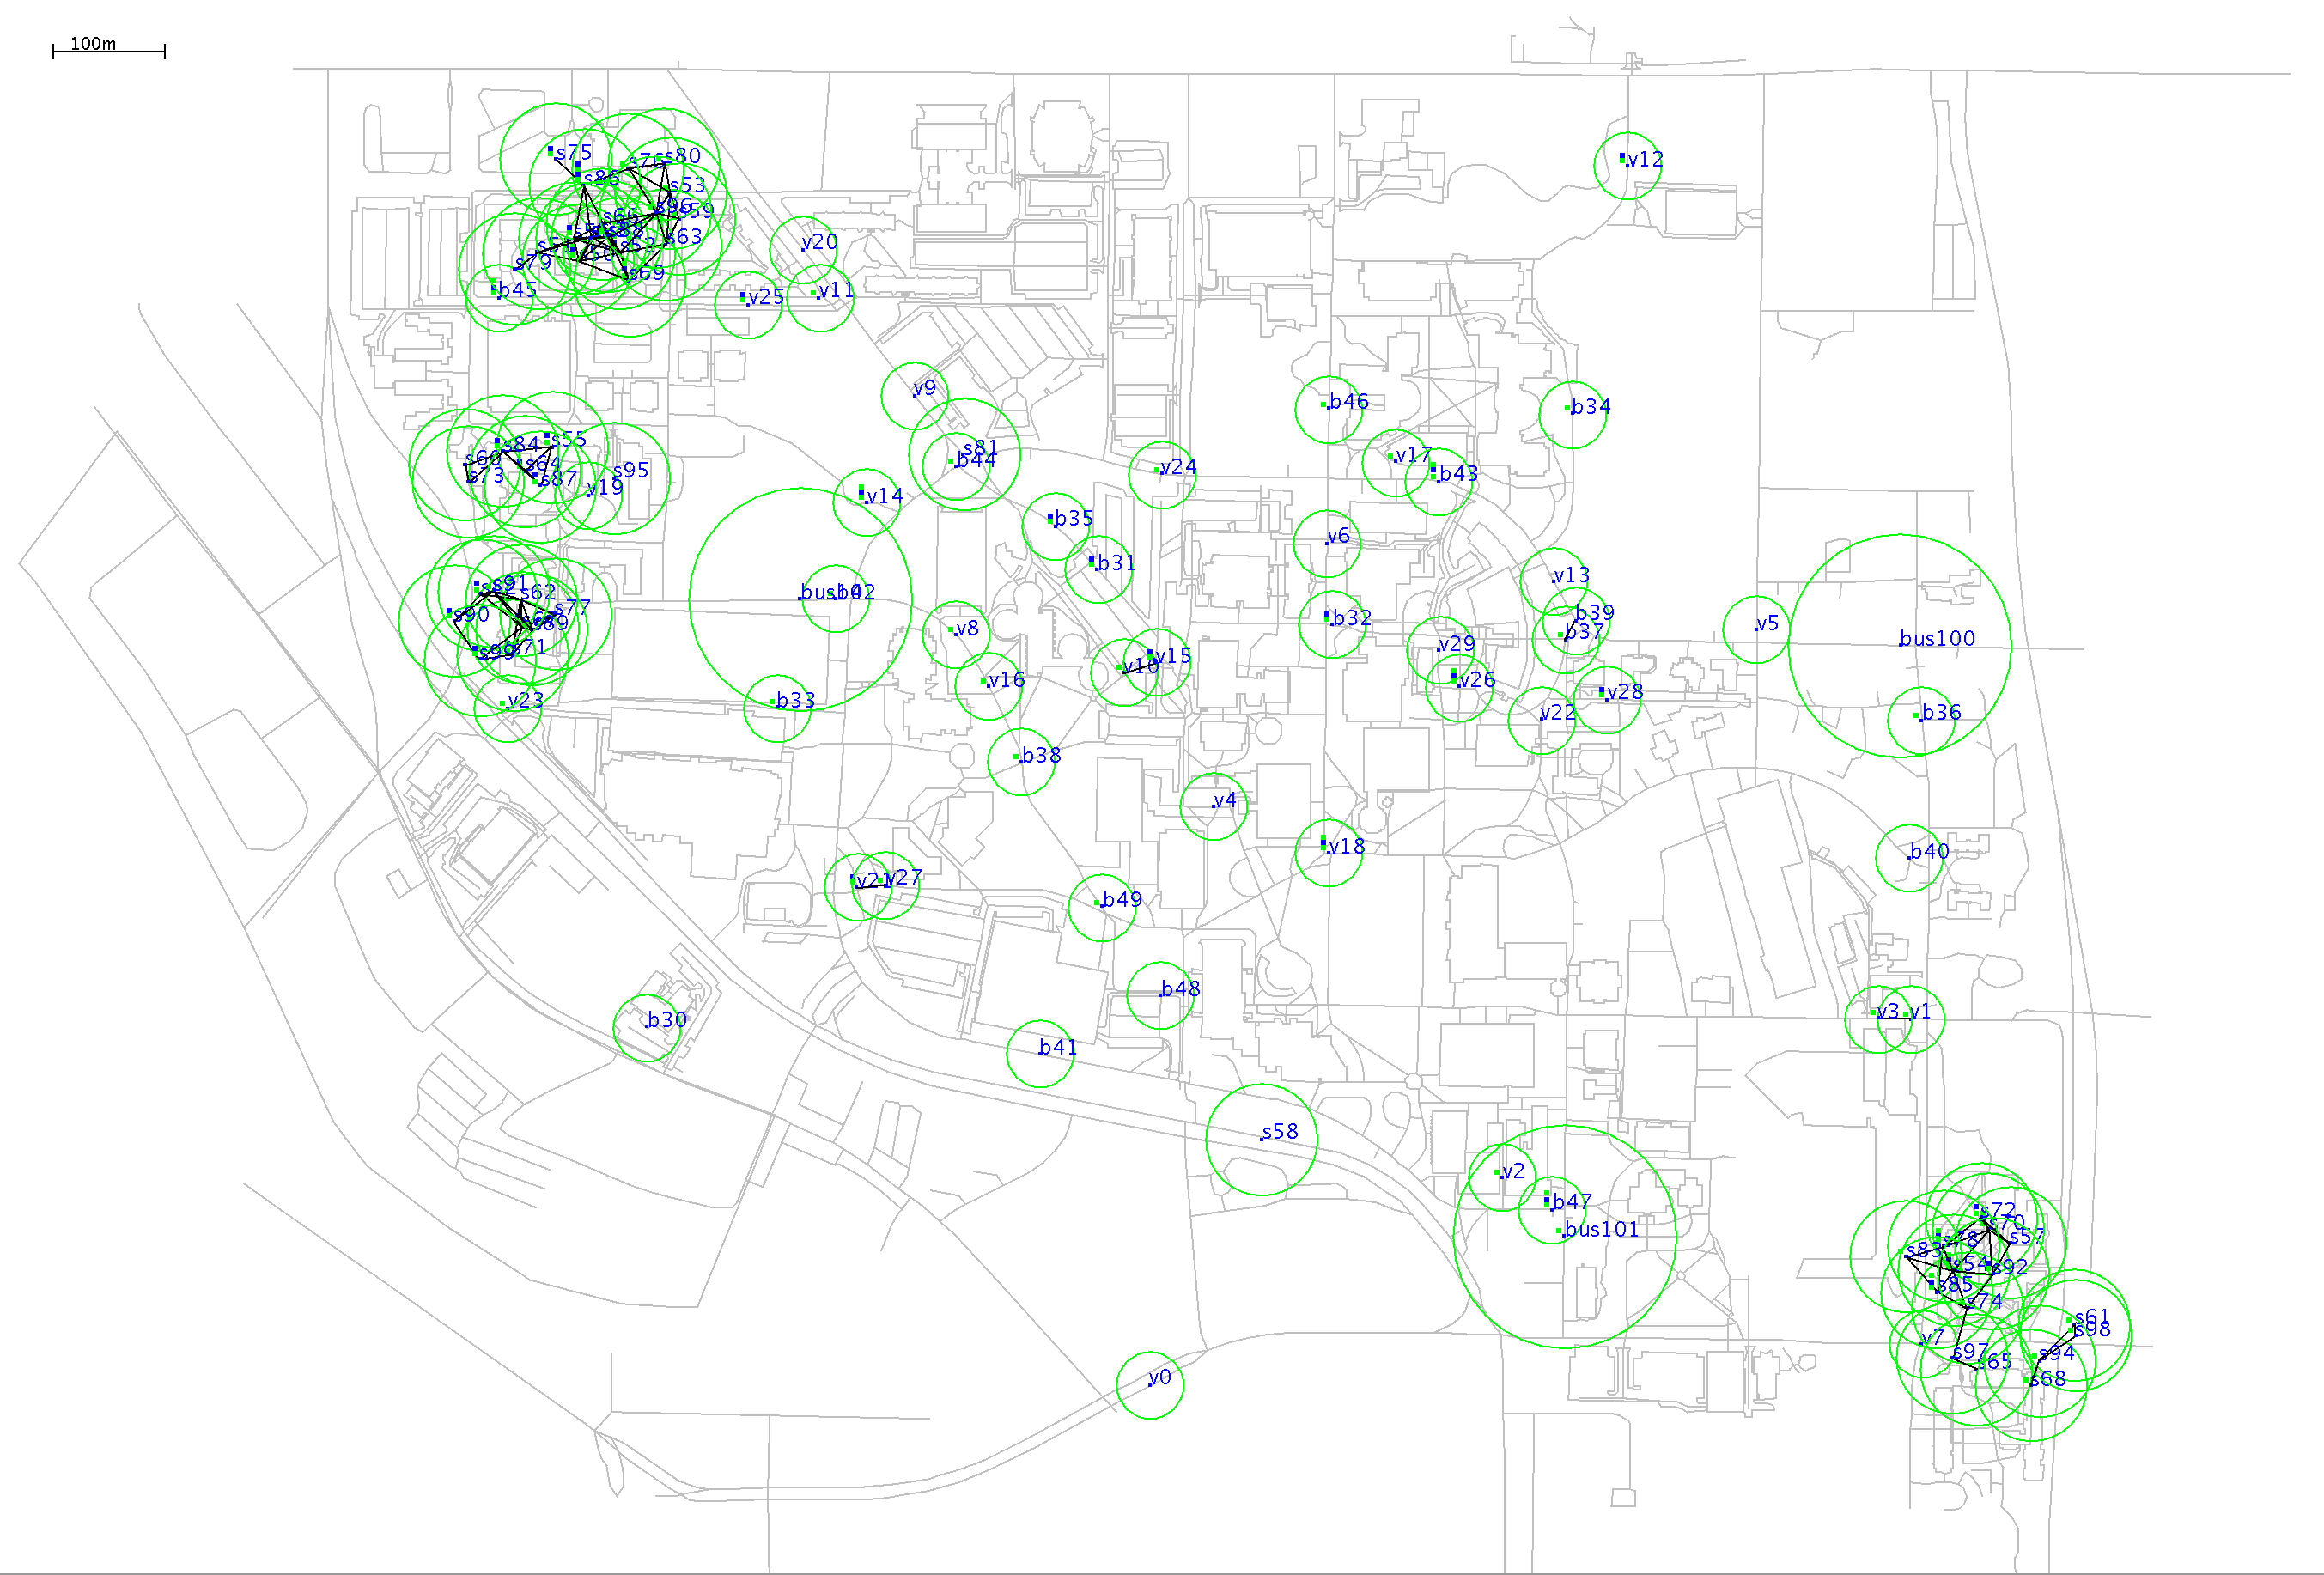
\includegraphics[width=3.5in]{simulation.png}
\caption{Running simulation based on the Georgia Tech campus}
\label{fig_simulation}
\end{figure}

\subsection{Bus route}

\begin{itemize}
  \item To make our simulation more interesting we decided to introduce a special group of nodes - buses.
  \item We focused on the GT red line bus since it is the only one that stays in bounds of our campus and its route is similar to other lines.
  \item The program OpenJUMP was used for the route selection.
  \item Unfortunately, it exported out many fragmented routes that had to be connected by hand, so the bus can go in one and circular way
\end{itemize}

\section{Networking hardware}

We specify 3 different network interfaces that can be used by nodes in our models. They all assume perfect circular transmission range.

\begin{itemize}
  \item Bluetooth 4.0: Speed = 750kB/s, range = 30 meters.
  \item Wifi direct: Speed = 7.5MB/s, range = 50 meters.
  \item Wifi direct+: Speed = 15 MB/s, range = 100 meters.
\end{itemize}

\section{Performance measurement methodology}

We evaluate different protocols in different situations using a variety of different measurements. Since nodes are mobile and will have a limited energy supply - except maybe buses, if they would use a generator from the engine rather than a battery - we want to consider different energy efficiency metrics.

The ONE simulator has some support for energy measurements in terms of how much energy the networking costs. Specifically, we are able to specify the initial energy level (i.e. battery capacity) and specify costs of transmission, scanning, scan response, and more. We have enabled the ONE to dump the current energy level of all nodes every hour (3600 seconds), and we use a separate script to generate the average energy level for each group of nodes. We will extend this to give other measurements such as used energy, number of nodes that ran out of battery, average (and maybe low, high) battery percentage remaining of nodes. We will use the resulting report to measure the energy efficiency of the different protocols.

The ONE simulator also supports other reports. Many of them are related to message delivery probability, statistics on queue sizes in the nodes, and total contact time (time within range of other nodes). Especially statistics on message delivery and queue sizes are the more straightforward performance measurements that we will compare between different protocols, although energy is also an important aspect in this setting.

\section{Node groups}

Nodes are the vital part of our simulation. They are basic communication units that can send, receive, buffer and route data. They are also subject to specified or stochastic movement with different speeds and directions. Every group of nodes uses a different network interface. We have four different groups with a total of 106 nodes. See the table \ref{node_groups}.

\begin{table}[!t]
\renewcommand{\arraystretch}{1.5}
\caption{Node groups}
\label{node_groups}
\centering
\begin{tabular}{|c||c||c||c||c|}
\hline
 & Visitors & Bikers & Students & Buses\\
\hline
Label & v & b & s & bus\\
\hline
Number & 30 & 20 & 50 & 3\\
\hline
Speed km/h & 0.5 - 1 & 2.5 - 3 & 0.5 - 1 & 4 - 5\\
\hline
Wait time s & 0 - 300 & 0 - 60 & 0 - 30 & 0\\
\hline
Movement & shortest p. & shortest p. & working day & route\\
\hline
Interface & BT & BT & Wifi direct & Wifi direct+\\
\hline
\end{tabular}
\end{table}

\section{Movement}

The basic movement type in the ONE simulator is ShortestPathMapBasedMovement. For each node, the simulator will randomly pick an end point on the map and move it there by using Dijkstra Shortest Path Algorithm.

In order to simulate the movement of different objects in real life, we decided to use two special movement types -- MapRouteMovement and WorkingDayMovement. They can help us easily control the movement pattern of different groups of nodes.

The MapRouteMovement model enables a group of nodes to follow a certain route which is defined by the user. In our experiment, it is applied to the bus group. By doing so, we can simulate the movement of Georgia Tech buses.

The WorkingDayMovement model presents the everyday life of average people that go to work in the morning, spend their day at work, and commute back to their homes in the evening. Some of them might go shopping afterwards.

We define multiple groups of people who work in different buildings and live in different apartments around the campus.

\section{Simulation results}

After running simulations, processing with post-simulation scripts and generating plots, we are able to compare the performance of the aforementioned protocols with respect to energy consumption, message delivery probability, message delivery statistics over time, and more. Let's dive in!

\subsection{Message delivery}

Let us start with the core concerns of protocols, namely whether or not they are good at delivering packets. The two main metrics we use to compare the protocols here is the probability that messages are delivered during the course of the day, and how long packets take to deliver, which we call they delay. Keep in mind that packets are created throughout the day rather than only at the beginning of day.

\begin{figure}
  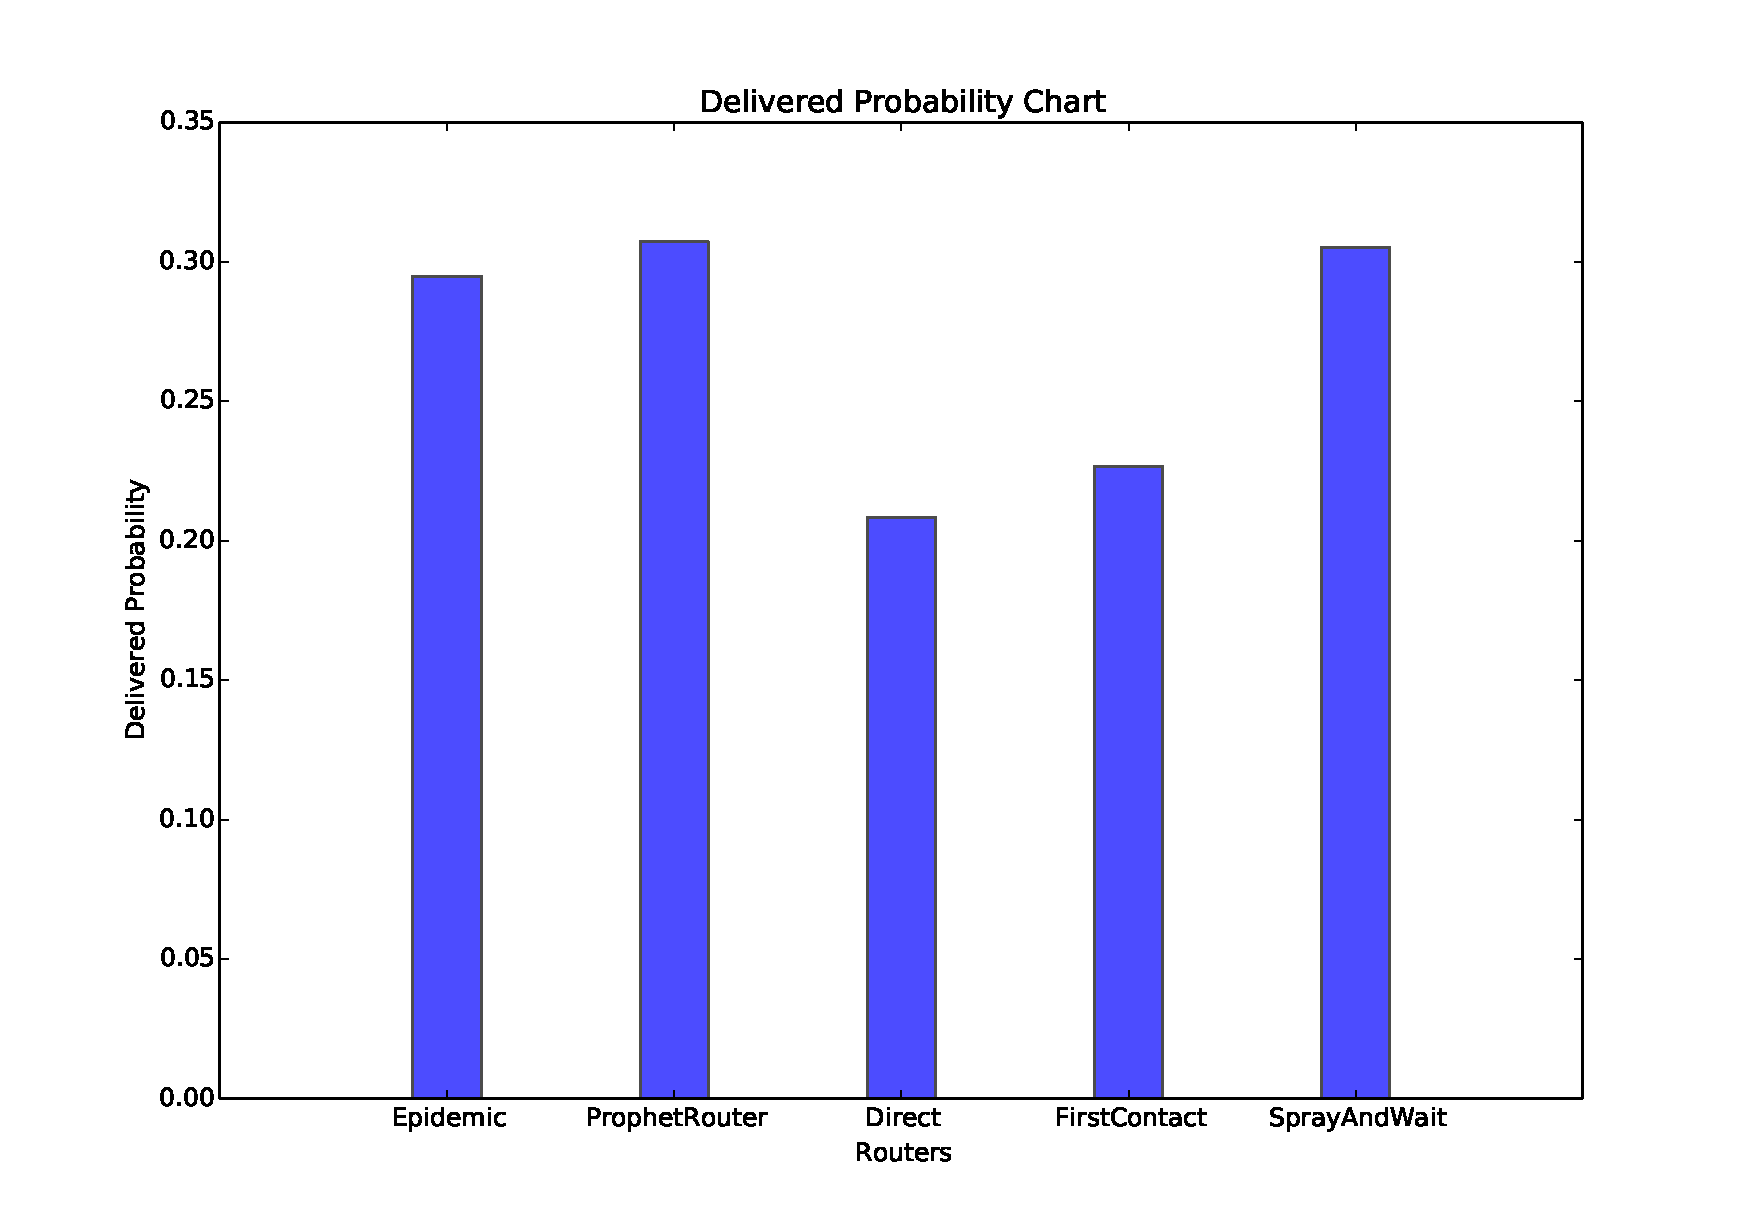
\includegraphics[scale=0.25, center]{../one_1.5.1-RC2/plots/delivered_prob.pdf}
  \caption{Delivered Package Probability}
  \label{fig:delivered_prob}
\end{figure}

\begin{figure}
  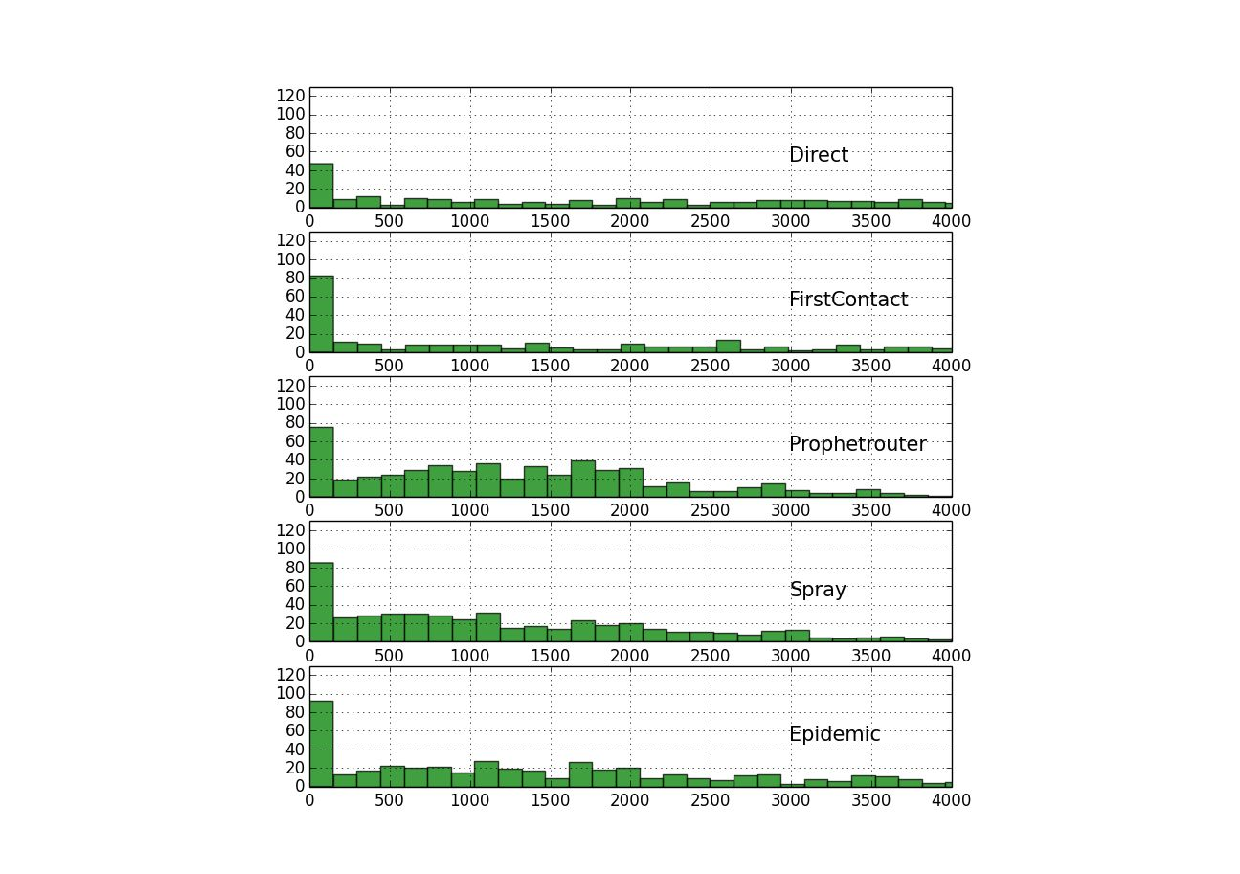
\includegraphics[scale=0.4, center]{../one_1.5.1-RC2/plots/Delivery_Time_Distribution.pdf}
  \caption{Delivery Time Distribution}
  \label{fig:time_distribution}
\end{figure}

Fig. \ref{fig:delivered_prob} is a comparison of the delivery probability of all messages for the protocols we are considering. We see that Spray and Wait, Epidemic and Prophet routing are distinguishing themselves from Direct and FirstContact routing by achieving more than five percentage points higher delivery probability. The difference between Spray and Wait, Epidemic and Prophet routing are only a few percentage points at most, so we would like to consider additional metrics to decide which protocol is better.

Fig. \ref{fig:time_distribution} shows the distributions of delivery time for each protocol. We can see from the chart that prophet routing has the best performance among all of the five protocols. Most of the delivered package can be transmitted to its destination within one hour.

\subsection{Energy efficiency}

Regarding energy efficiency, the ONE gives us the energy level of every node in a certain interval. In our simulations we have used 1200 second intervals, i.e. every 20 minutes of simulated time. We then process this information to generate statistics by node group over time, such as average energy consumption and average battery percentage remaining. Let us consider the average energy consumption of different node types under the protocols we consider.

\begin{figure}
  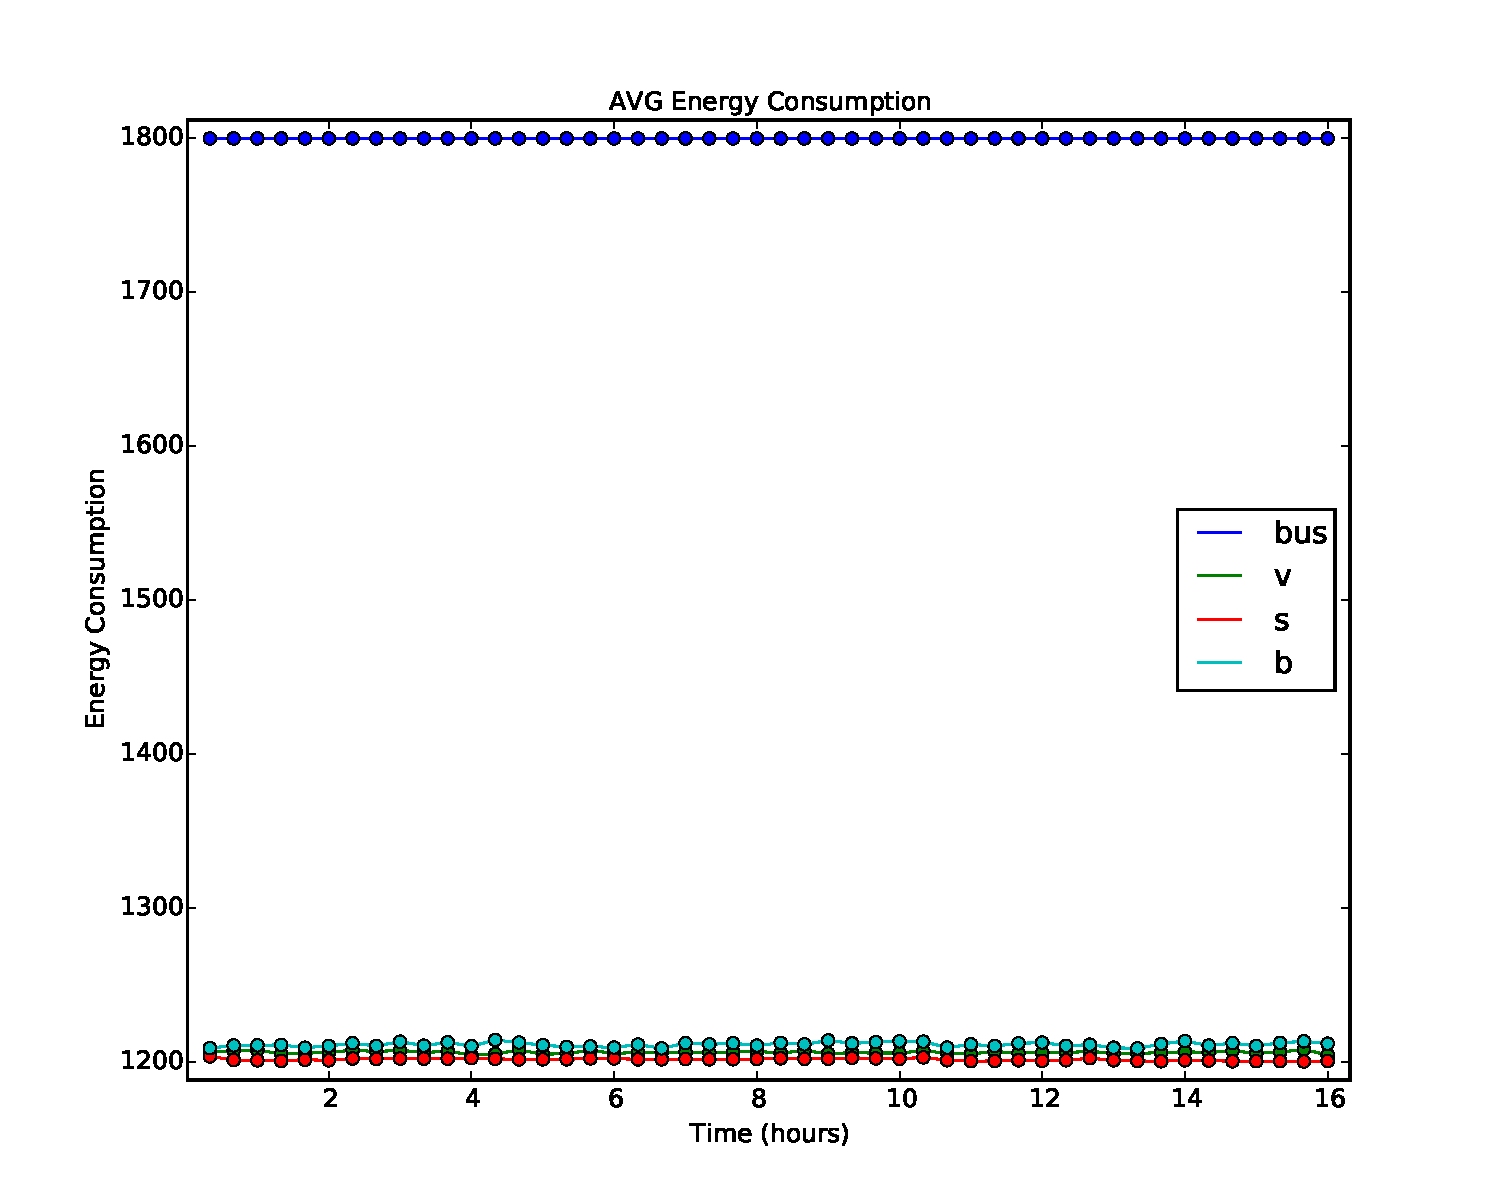
\includegraphics[scale=0.25, center]{../one_1.5.1-RC2/plots/SprayAndWait_AVG_ENERGY_CONSUMPTION.pdf}
  \caption{Average energy consumption, Spray and Wait routing}
  \label{fig:avg_consumpt:snw}
\end{figure}
We see in fig. \ref{fig:avg_consumpt:snw} that while the buses have a relatively high energy consumption, the levels are stable for all groups over the whole simulation. Let's consider some other protocols to get an idea of how Spray and Wait compares to the other protocols.

\begin{figure}
  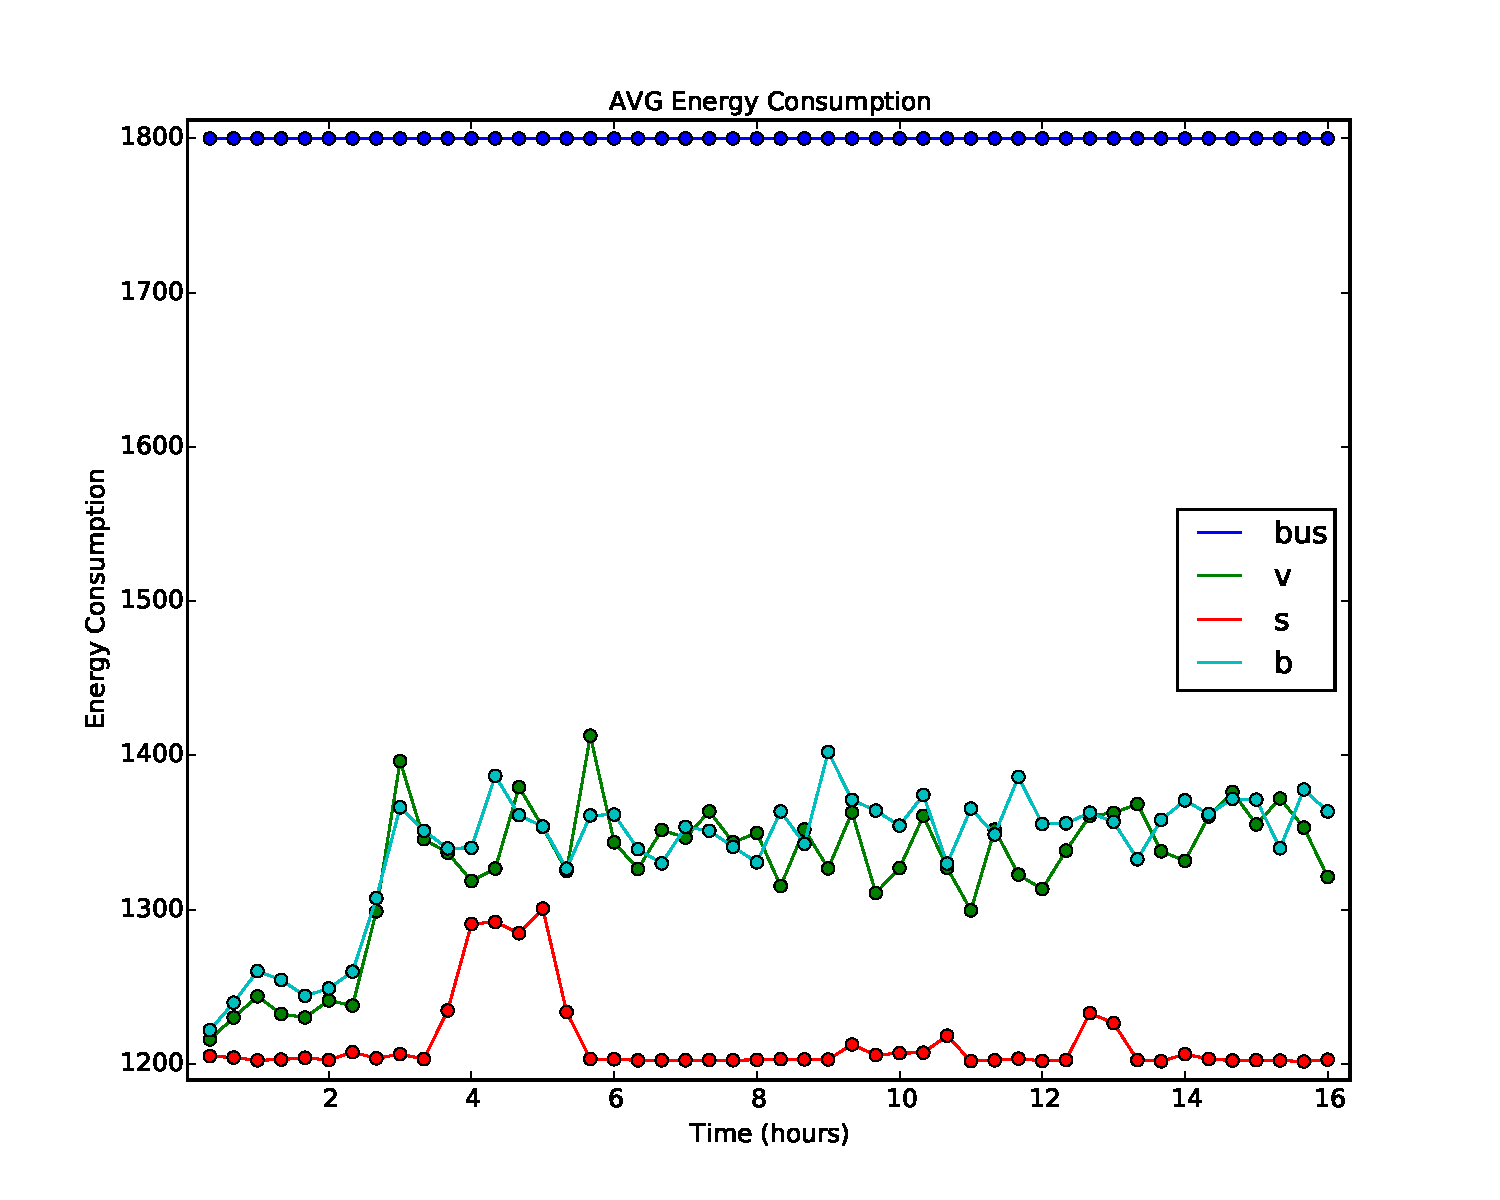
\includegraphics[scale=0.25, center]{../one_1.5.1-RC2/plots/Epidemic_AVG_ENERGY_CONSUMPTION.pdf}
  \caption{Average energy consumption, Epidemic routing}
  \label{fig:avg_consumpt:epidemic}
\end{figure}

With Epidemic routing, in fig. \ref{fig:avg_consumpt:epidemic}, energy consumption reaches higher levels for both visitors and bikers, with occasional peaks in the energy consumption of the students. How come we see these peaks? Let's take a look at the amount of packets that are being sent.

\begin{figure}
  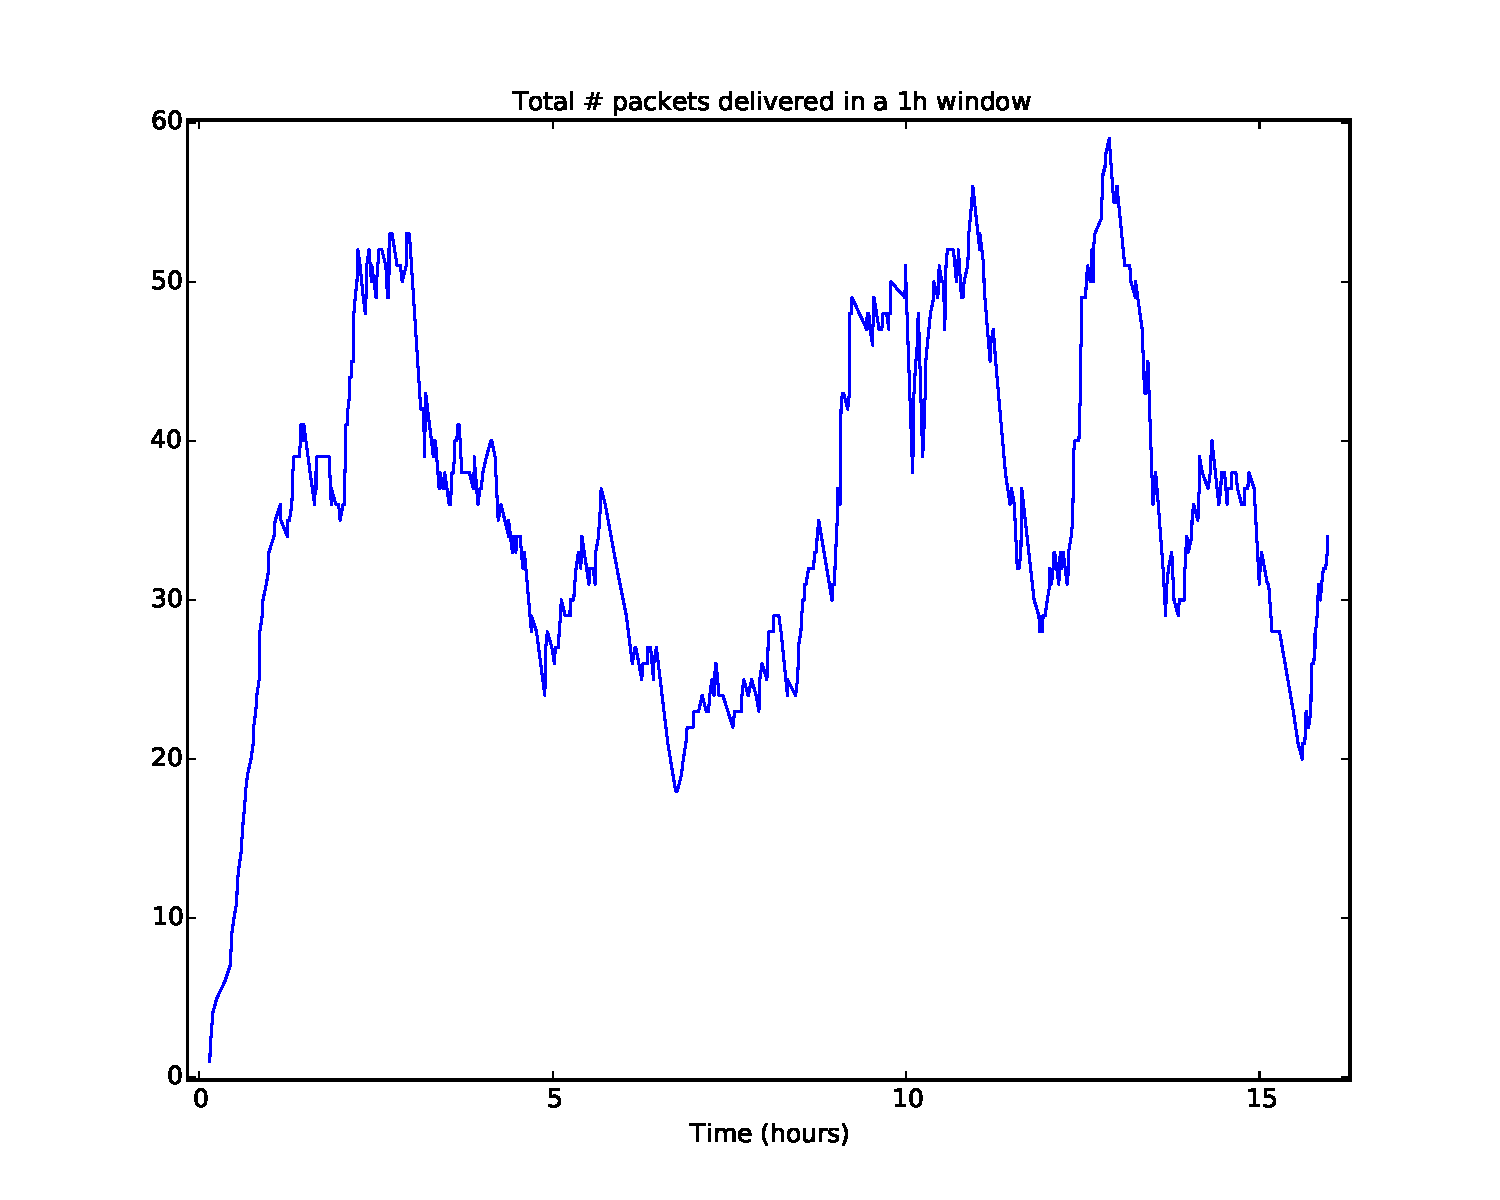
\includegraphics[scale=0.25, center]{../one_1.5.1-RC2/plots/Epidemic_NUM_DELIVERED_PKTS_IN_WND.pdf}
  \caption{Number of packets delivered in the last hour, Epidemic routing}
  \label{fig:pkts_in_wnd:epidemic}
\end{figure}

Fig. \ref{fig:pkts_in_wnd:epidemic} shows the number of packets sent within the last hour, at any point in time, when Epidemic routing is used. We see some peaks that we can link to the two peaks that we saw in the students' energy consumption! But what about Spray and Wait, why are there no peaks in their energy consumption?

\begin{figure}
  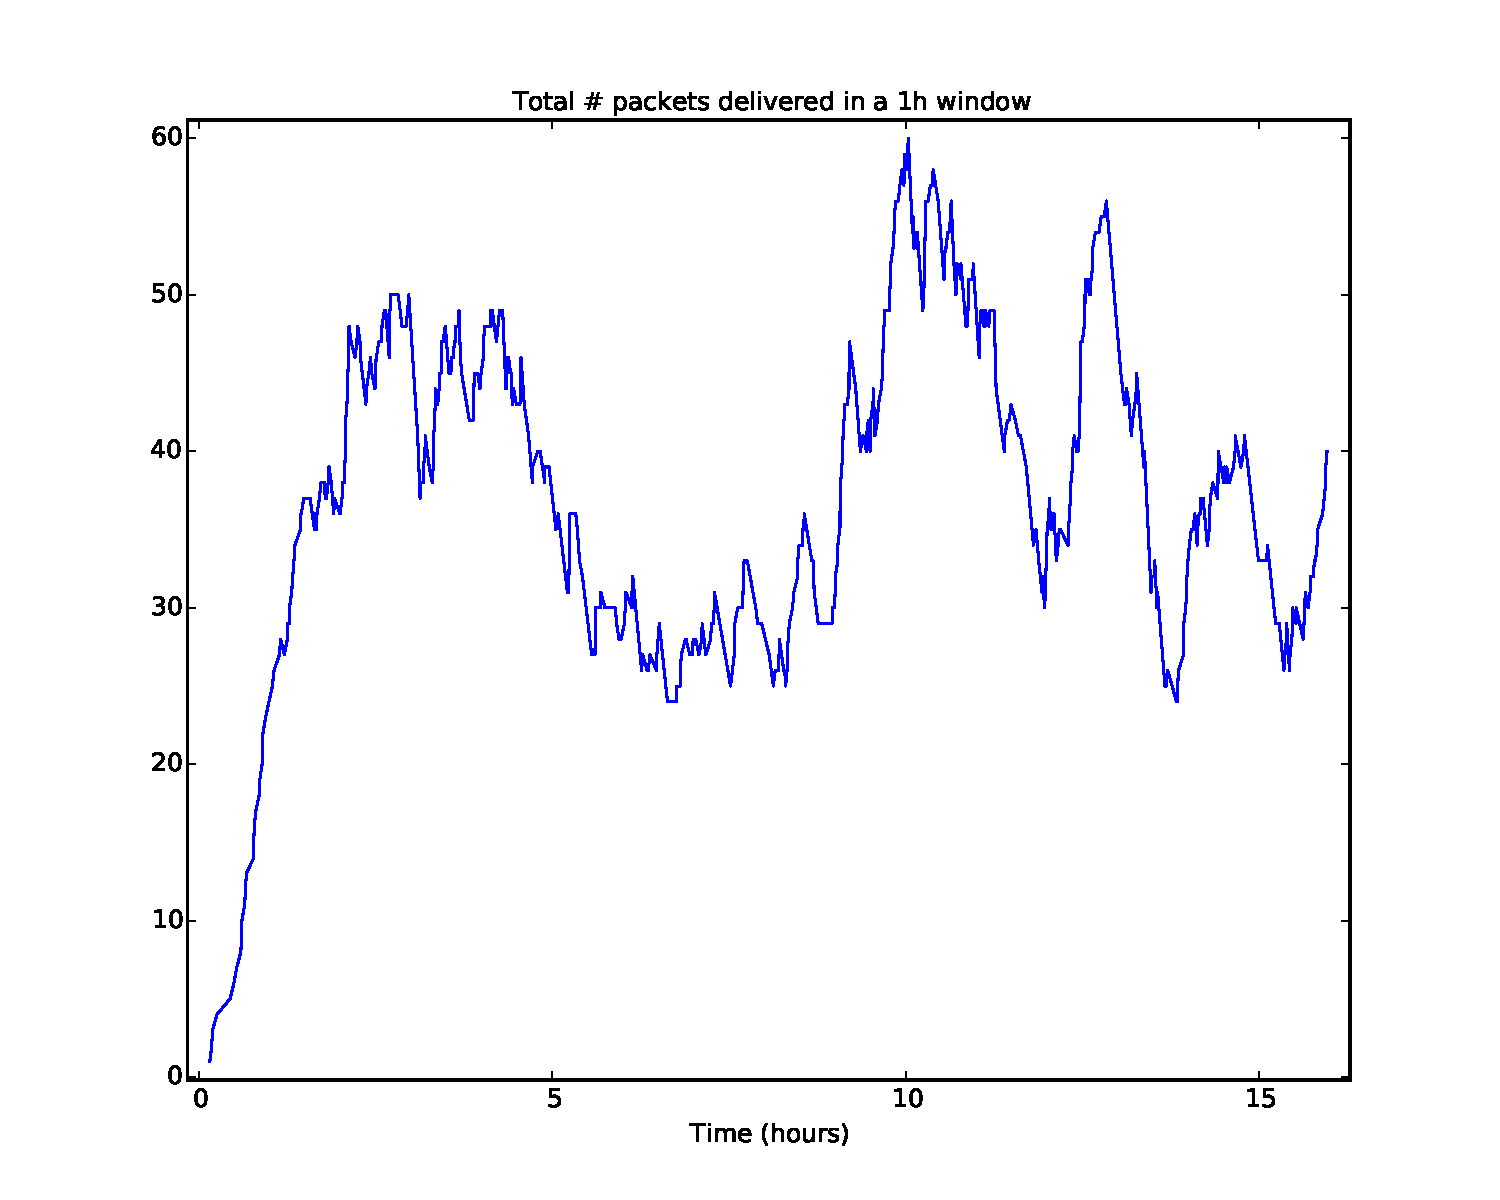
\includegraphics[scale=0.25, center]{../one_1.5.1-RC2/plots/SprayAndWait_NUM_DELIVERED_PKTS_IN_WND.pdf}
  \caption{Number of packets delivered in the last hour, Spray and Wait routing}
  \label{fig:pkts_in_wnd:snw}
\end{figure}

In fig. \ref{fig:pkts_in_wnd:snw} we see very similar peaks, in fact, although they seem to deviate slightly less from the average. But given that the energy consumptions are so different, it seems safe to conclude that Spray and Wait is more energy efficient. Let's have a look at the average energy consumption when Prophet routing is used.

\begin{figure}
  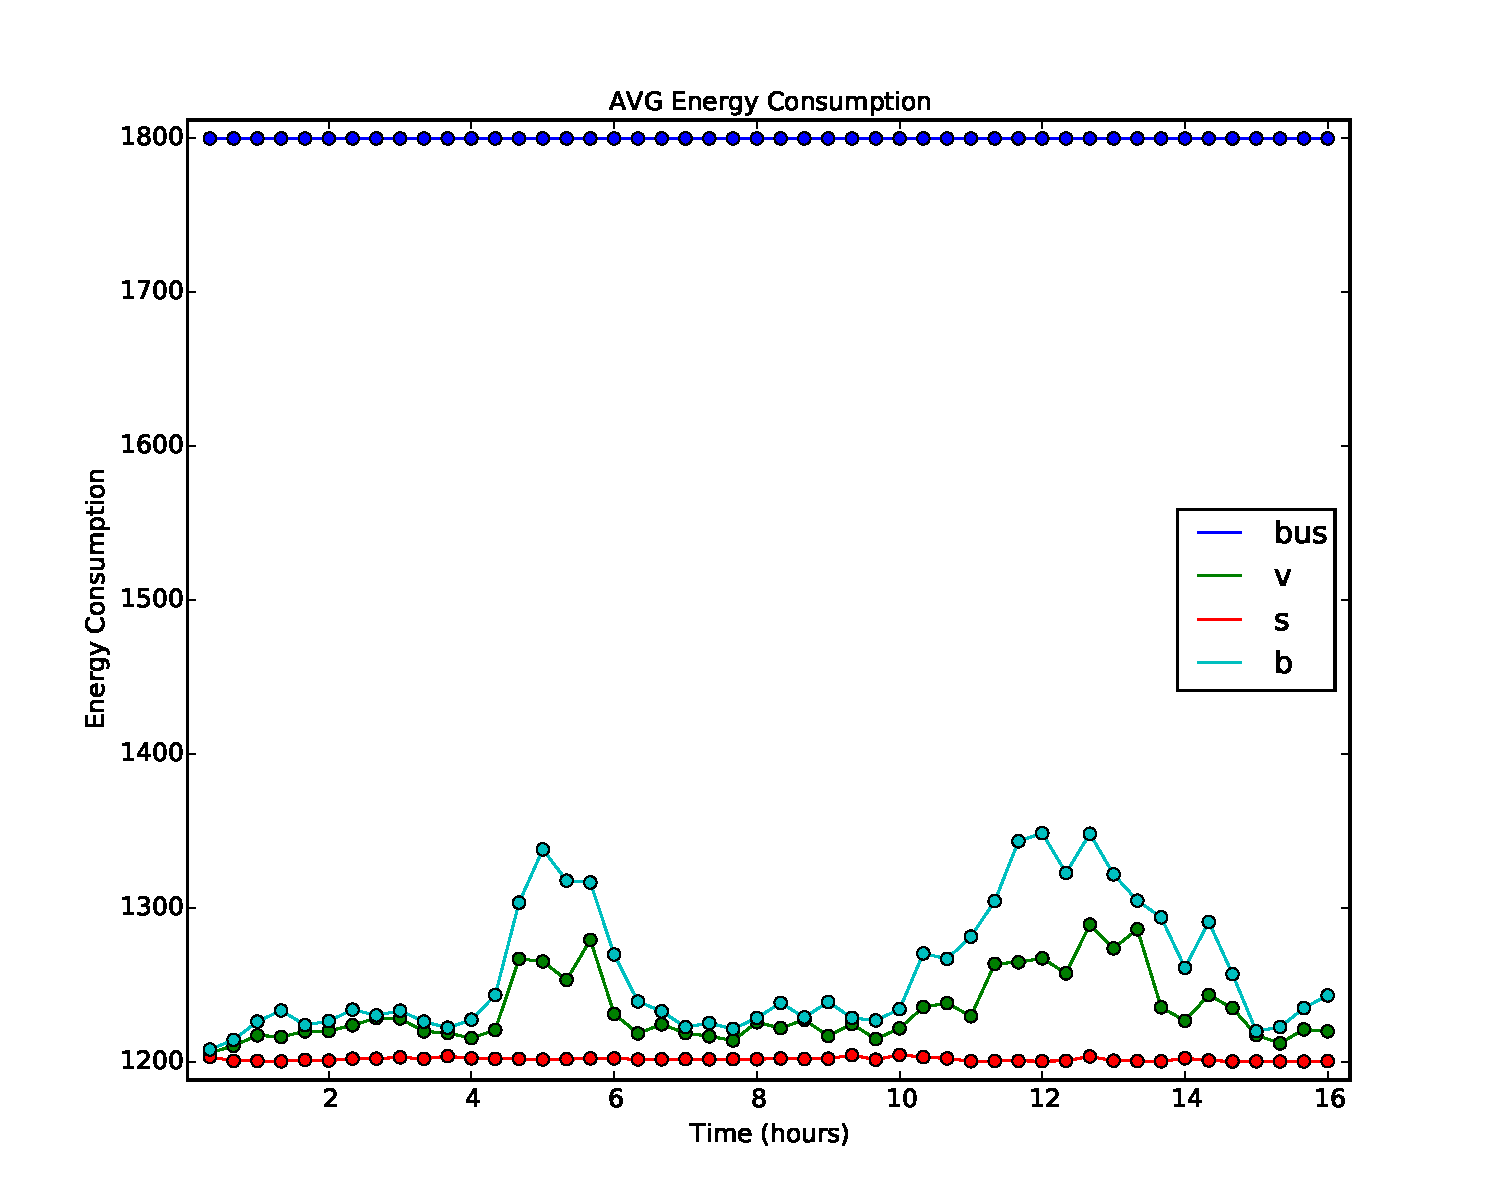
\includegraphics[scale=0.25, center]{../one_1.5.1-RC2/plots/ProphetRouter_AVG_ENERGY_CONSUMPTION.pdf}
  \caption{Average energy consumption, Prophet routing}
  \label{fig:avg_consumpt:prophet}
\end{figure}

Interestingly enough, the students' energy consumption is flat in fig. \ref{fig:avg_consumpt:prophet}, while the visitors have peaks in roughly the same time periods as Epidemic routing had! Even with the peaks, though, the energy consumption of visitors and bikers is on average lower than that of Epidemic routing, and higher than with Spray and Wait. It seems like Spray and Wait and Prophet routing are good protocols in our scenario, given that Prophet routing had slightly higher message delivery probability.

Let's assess the energy consumptions of the protocols that struggled more in terms of message delivery probability, namely Direct routing and FirstContact routing.

\begin{figure}
  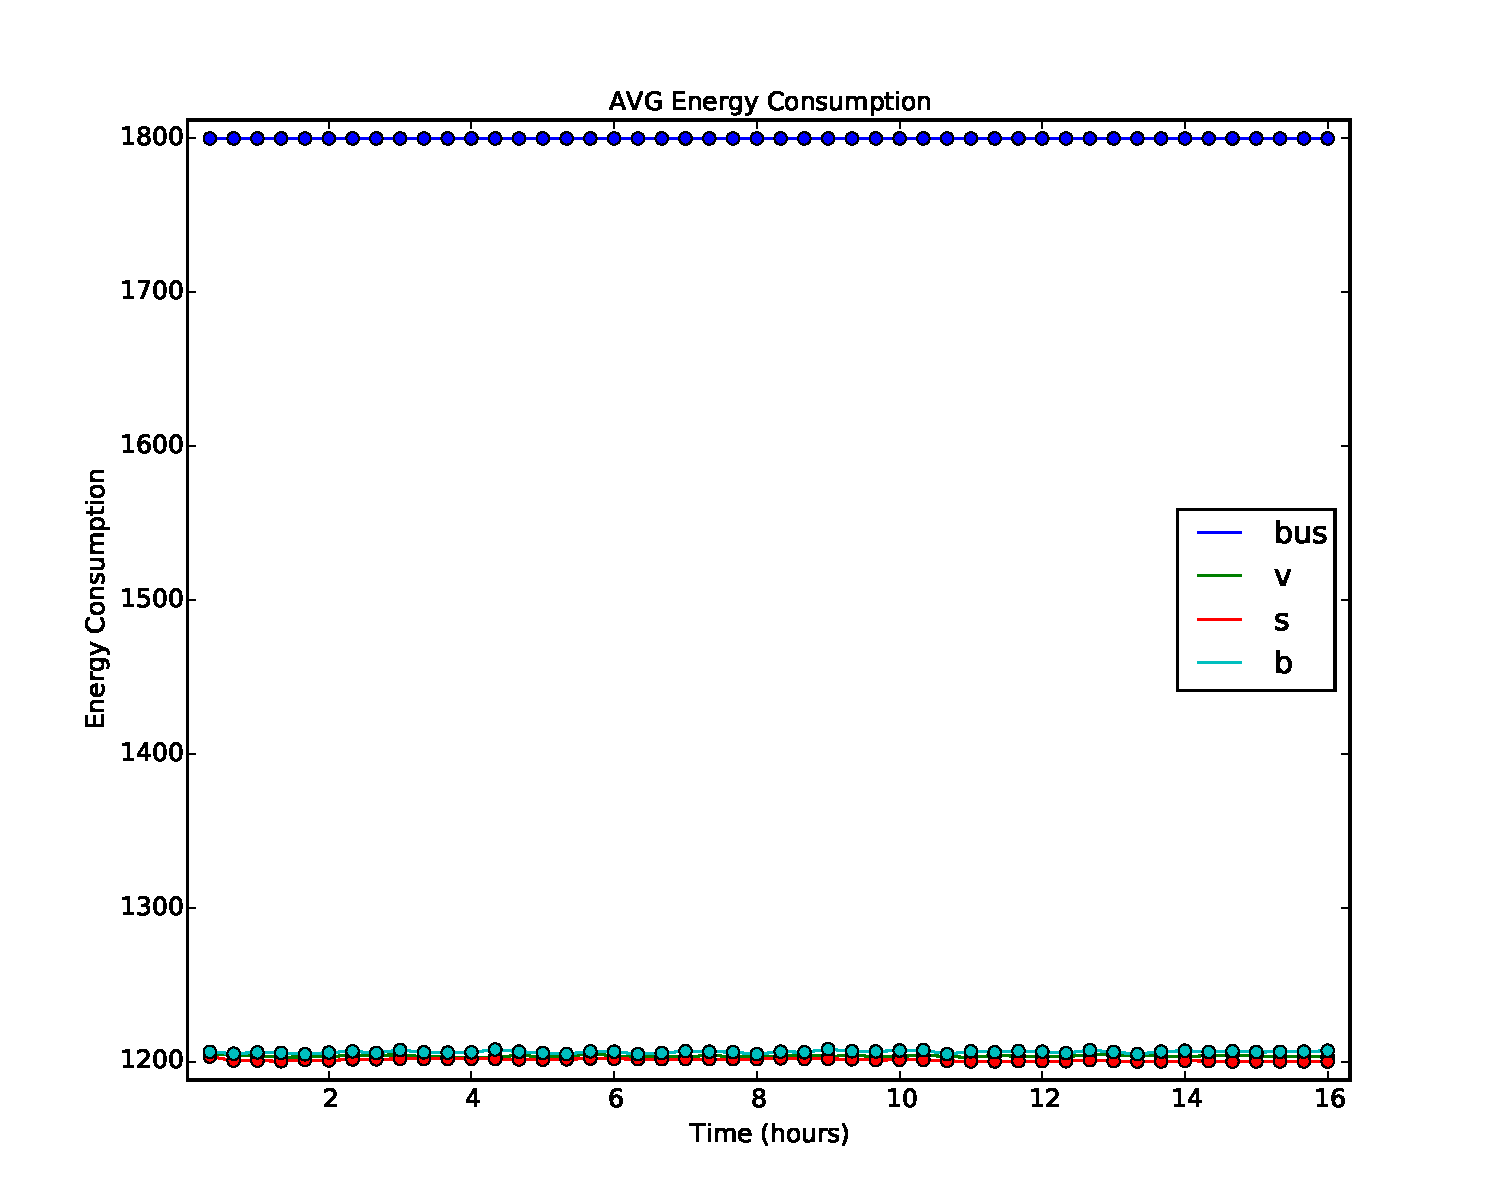
\includegraphics[scale=0.25, center]{../one_1.5.1-RC2/plots/Direct_AVG_ENERGY_CONSUMPTION.pdf}
  \caption{Average energy consumption, Direct routing}
  \label{fig:avg_consumpt:direct}
\end{figure}

We see in fig. \ref{fig:avg_consumpt:direct} that Direct routing's performance in terms of energy consumption. As it turns out, this is the least energy consuming protocol that we consider - the visitors and bikers are slightly lower than with Spray and Wait.

\begin{figure}
  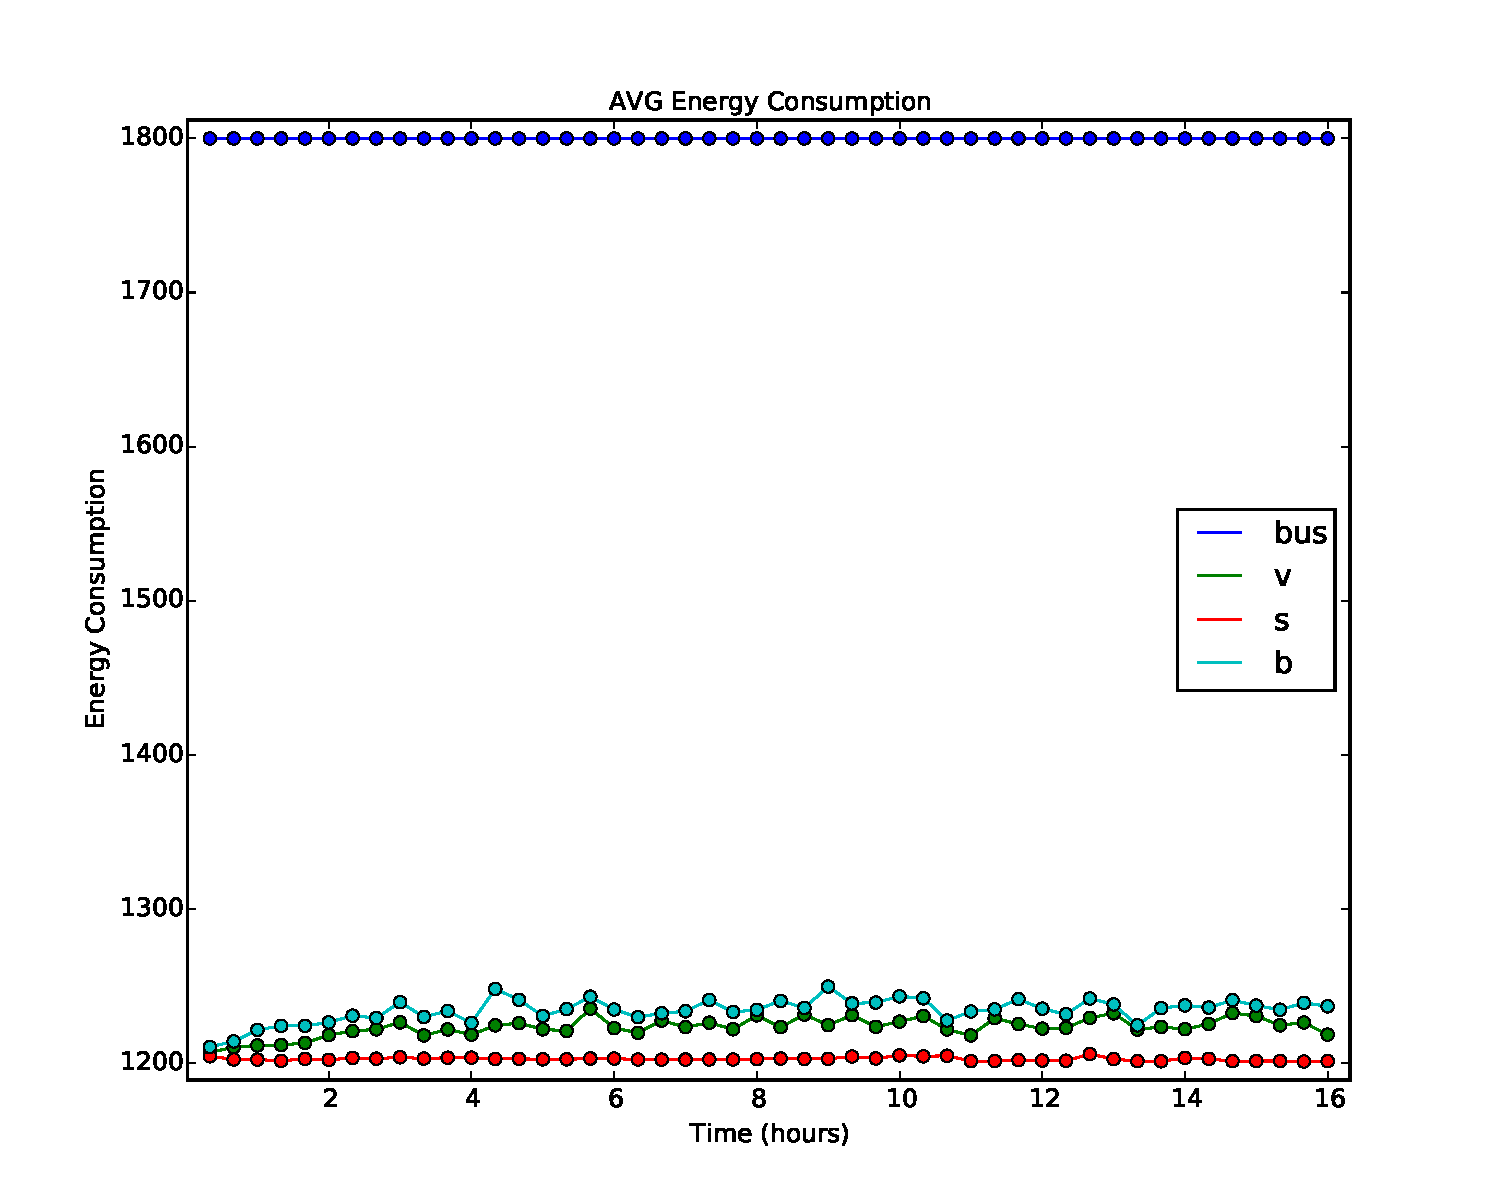
\includegraphics[scale=0.25, center]{../one_1.5.1-RC2/plots/FirstContact_AVG_ENERGY_CONSUMPTION.pdf}
  \caption{Average energy consumption, FirstContact routing}
  \label{fig:avg_consumpt:firstcontact}
\end{figure}

We see in fig. \ref{fig:avg_consumpt:firstcontact} that with FirstContact routing the consumption is lower and more stable than using Epidemic or Prophet routing, but not quite as good as Direct or Spray and Wait routing. Still, this is not a large difference from them by any means, and thus FirstContact is also a protocol that consumes a bit less energy.\\

{\color{red}
  TODO more analysis, else write some conclusions? Maybe as below:
}
From our findings in this section, it seems like Prophet routing and Spray and Wait are the best choices in our scenario. Prophet routing provides slightly higher message delivery probability at a cost of slightly higher and less consistent energy consumption than that of Spray and Wait. Which protocol would be best is simply a matter or what is most important in a given application - slightly longer battery time, or higher probability that a message arrives during the day it was created.

% conference papers do not normally have an appendix

% use section* for acknowledgement
\section*{Acknowledgment}

We would like to show our gratitude to Dr. Mostafa Ammar, Georgia Tech for sharing his pearls of wisdom with us during the Computer Networks course and his guidance received while working on this project.

\bibliographystyle{unsrtnat}
\bibliography{refs}

% that's all folks
\end{document}


